\documentclass[m,intern,palatino]{cgBA}
\author{Maximilian Luzius}
\title{Markerloses Tracking mithilfe Analyse durch Synthese auf Basis eines Partikelfilters}
\zweitgutachter{Anna Katharina Hebborn, M.Sc.}
\zweitgutachterInfo{(Institut f�r Computervisualistik, AG Computergraphik)}
%\externLogo{3cm}{logos/UniLogoNeu}
\externName{Computervisualistik}

\begin{document}

% Umschalten der Sprache (f�r englische Rubrikbezeichnungen etc.)
%\selectlanguage{english}


\maketitle

\pagenumbering{roman}
\newpage
\tableofcontents
\clearpage         % oder \cleardoublepage bei zweiseitigem Druck
% \listoffigures   % fuer ein eventuelles Abbildungsverzeichnis
% \clearpage
\pagenumbering{arabic}

% Hier kommt jetzt der eigentliche Text der Arbeit

\section{Einleitung}

Im Bereich der Augmented Reality(kurz AR) wei�t Tracking, besonders markerloses Tracking, eine der gr��ten Schwierigkeiten auf. Unter Augmented Reality wird verstanden, dass ein Kamerabild durch synthetische Informationen in Echtzeit �berlagert oder auch erg�nzt wird, so dass die Realit�t erweitert wird. Damit diese synthetischen Informationen an den richtigen Stellen eingeblendet werden k�nnen, muss aus der Sicht der realen Welt bestimmt werden, wo sich die Kamera befindet(Position) und wo sie hin blickt(Orientierung), die sogenannte Kamerapose. Im Bereich der AR gibt es zwei Herangehenswei�en, die in markerloses und markerbasiertes Tracking unterteilt werden, jedoch meist beide nur in speziell vorgesehenen Bereichen funktionieren. Au�erdem werden diese h�ufig durch 3D-Modelle der Umgebung und der Objekte unterst�tzt. Beim zweiten Verfahren werden in die reale Welt Marker(Bit-Codes z.B. QR-Code) eingef�gt, so dass deren Position und Gr��e bekannt ist und diese von der Kamera erkannt werden k�nnen und folglich die Kamerapose zur�ckgerechnet werden kann. Das Problem dieses Verfahrens sind die Marker, welche vorher in der Welt angebracht werden und in dieser auch gut sichtbar sein m�ssen. Somit wird das markerlose Trackingverfahren immer wichtiger und sollte, soweit m�glich das markerbasierte ersetzen. Da dieses Trackingverfahren f�r die Arbeit von bedeutung ist, werden verschiedene Ans�tze in den Grundlagen vorgestellt...ADS und/oder SLAM?....

\section{Grundlagen}
\subsection{Modellbasiertes Tracking}
\subsection{Markerloses Tracking}
\subsection{Analyse durch Synthese}
Diese Methode setzt vorraus, dass ein exaktes 3D-Modell der Umgebung vorhanden ist. Desweiteren ist eine initiale Pose n�tig, so dass die Methode wei�, an welcher Stelle sich die Kamera im Weltkoordinatensystem zu Begin befindet. Auf dessen Basis wird das aktuelle Kamerabild errechnet, indem die Pose des vorherigen bekannt ist und in deren n�chster Umgebung(nach Gau�?) neue synthetische Bilder gerendert werden. Diese werden mit dem aktuellen Bild entweder merkmals- oder �hnlichkeitsbasiert abgeglichen, so dass das synthetische Bild mit der h�chsten �hnlichkeit die neue Kamerapose ist.

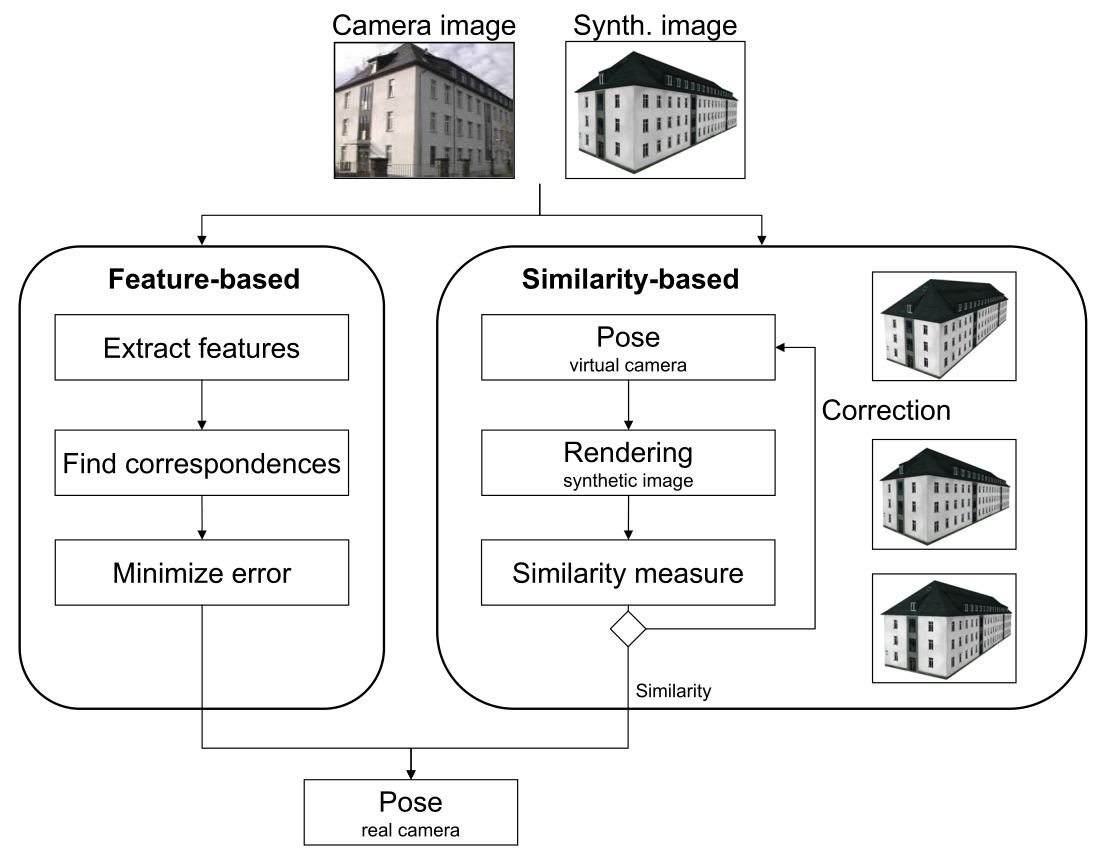
\includegraphics[scale = 0.33]{bilder/ADS}
\begin{center}
\textit{Abb.1: ADS Schema}
\end{center}

\subsection{Partikelfilter}
Der Partikelfilter ist ein System um in diesem Fall die sich bewegende Kamerapose neu zu sch�tzen. Es funktioniert in der Weise, dass um die letzte bekannte Pose eine Partikelwolke mithilfe der Dichtefunktion aufgespannt wird, wobei aus der Sicht eines jeden Partikels ein synthetisches Bild gerendert wird(wdh. von ADS, lieber allgm. fassen?)  

\section{Stand der Technik}
Definition des �hnlichkeitsma�es(Schwellwertes), Vergleichsarten -> recherche, Sebastian Kowalzky Houghtransformation war nix

\section{Fragen}
-Grundlagen nach und nach erg�nzen? Ja
\newline -Der oder das Filter? Das Filter
\newline -Nicht zu viel vorstellen(andere Methoden, besonders markerbasiert eher nicht), da nur BA-Arbeit? Verfahren wie Partikelfilter nicht so ausf�hrlich wie MNohn? -Markerbasiert nicht, kein SLAM, Partikelfilter recht ausf�hrlich
\newline -Abb. aus Prim�rliteratur referenzieren?! Ja
\newline -Partikelfilter in Aufbau nach ADS? Ja. Benutzt der Partikelfilter nur die letzte Pose oder auch die Bewegungstendenz der vorherigen? Beides, kommt auf die Implementierung an
\newline -Was geh�rt zu ADS, auch Gau� oder Partikelfilter? ADS ist rendern und vergleich
\newline -ADS sowohl merkmals- als auch �hnlichkeitsbasiert vorstellen? Ja. Umsetzung aber �hnlichkeitsbasiert(kanten) oder freie Wahl? Ja.
\newline -Welches Betriebssystem? Windows
\newline -Wann bist du in Singapur? August-Oktober
\newline -Edge based Tracking blob anschauen

\subsection{1.1}
-lineare verfahren -> Merkmalskorrespondenzen
\newline -nichtlineare verfahren -> �hnlichkeitsbasiert
\newline - Analyse auf Kantenbildern mithilfe der Teabox -> Haus/Stadt
\newline - Schwarz-Wei� Eingabebild?
\newline - Sobeloperator zur Kantendetektion -> sieht gut aus
\newline - Cannyoperator nur ein Pixel breite Kante -> Dilatation verst�rken?
\newline -Hough-Transformation braucht parametrisierbare Form
\newline - Webcam vom Laptop oder externe? Video -> Aufl�sung 800x600
\newline - Qt und OpenCV?Ja

\end{document}